\subsection{Connected Cyber-Physical Systems}

Connected systems is not a new concept; however, it is used more than ever in today’s day and age, even on a personal basis. There are hardly any personal electronic devices which are used independently without being connected to a system, or the internet. This phenomenon is not just limited to personal systems and is also prevalent in other industries like heavy machinery, automobiles, etc., where every individual system is connected to one or more systems, which monitors or controls them according to the requirement. For instance, Vivint.com [1] competently describes smart home, as a home that is equipped with technology to remotely control and automate household systems like lighting, doors, thermostats, entertainment systems, security alarms, surveillance cameras and other connected appliances. The Internet of Things (IoT) can be described as a system that includes the collection of tangible components that are connected, either wirelessly or otherwise, and the system is connected to internet. The components may include a range of sensors which can use various types of local area connections such as RFID, NFC, Wi-Fi, Bluetooth and Wide Area Connectivity, such as GSM, GPRS, 3G and LTE, and can record human or other activities which can then be relayed to another component, such as the processing system, and this information can be used to operate the system effectively, to gather data, to troubleshoot the system, or to perform any other relevant tasks. [2]. The deployment diagram of a typical IoT system is shown in Figure I 1. Multiple connectivity between entities can be observed. Some devices are connected wirelessly where as some have a wired connection. Moreover, all the sub-systems belong to different manufacturers. However, all of them work together to form an orchestration.

\begin{figure}[h]
	%\begin{framed}
	\centering
	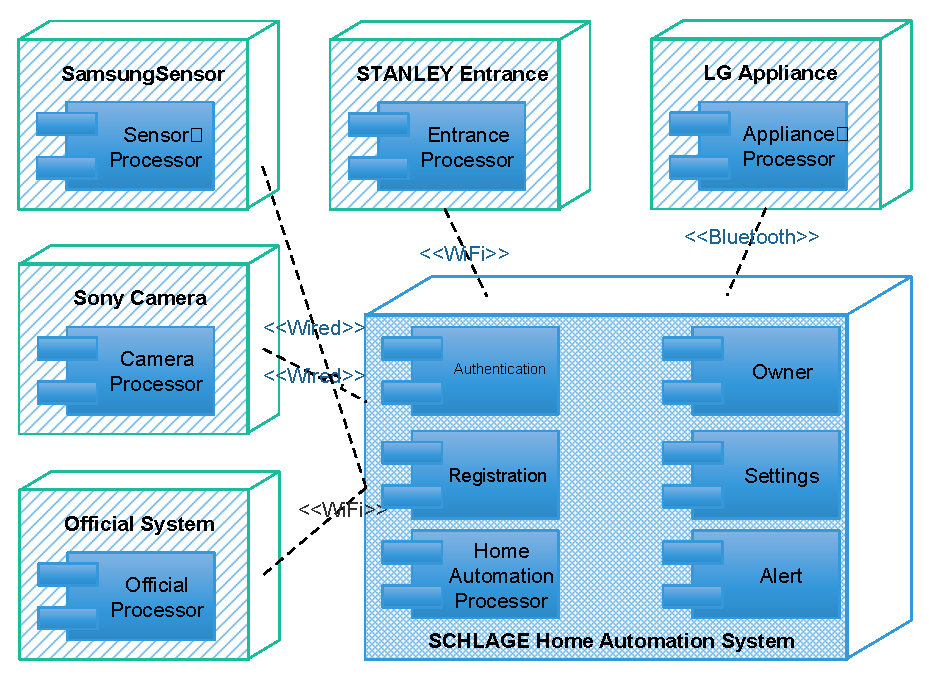
\includegraphics[width=\columnwidth]{images/shdd.eps}
	\caption{A Typical Smart Home Deployment Diagram.}
	\label{fig:SmartHomeDepDiagram}
	%\end{framed}
\end{figure}

Like the Figure I 1, more often than not, most of the components in an IoT system are manufactured by different vendors. Though many failures within an individual component may be taken care of by their respective manufacturers; however, it is likely that any other failure between different components in an IoT system, such as a simple connectivity problem will not be supported by the manufacturers, as it is generally not covered under the warranty. A popular report from Forrester [3] predicts that there will be a huge growth in the IoT industry in the next years where enterprises will increase their efforts to introduce voice-based services to consumers and new European guidelines will allow commercializing the IoT data. In 2010, the number of objects connected to the Internet surpassed the earth’s human population [4]. Additionally, Symantec [5] predicts that there will be up to 21 billion connected devices by 2020, and not just the consumers, but cities and companies will also start adopting smart technologies in their operations. A report from Gartner [8] says that the worldwide spending in IoT Security was 1.1 Billion USD and it is projected to skyrocket at more than 3.1 Billion USD in 2021, which is a direct result of the increase in vulnerabilities in the systems.

The above discussion leads us to believe that diagnosing and troubleshooting failures in an IoT system will be a huge problem in the near future which may not be covered by any manufacturer, unless all the entities within the system are manufactured by the same company. In this paper, we will address the issue of IoT self-healing that is automatically diagnosing and troubleshooting IoT systems. Other related concepts such as error prevention will also be looked at. This field has been prolifically researched over the years under various other lexical analogues, one of them being Self-Healing [9][10][11]. Several surveys have been done previously on Self-Healing [30][9][31][32], however, they do not specifically discuss the phenomenon for IoT.

There are many ways to detect if an error has occurred in a system [34]. One of them is System-Level Monitoring that is used by several commercial enterprise applications. Another notable method is to detect errors/failures at the application layer. However, the most common way to examine a system for detecting any error, fault or failure is by analyzing the event logs generated by the system. Therefore, in this paper, we will focus on the research works that emphasize on analyzing event logs for detecting and diagnosing errors.

The organization of this paper is as follows: IoT error prevention detection and diagnosis will be briefly surveyed in Section II. Specific methods for log analysis and process mining will be addressed in Section III. Finally, Section IV will draw conclusions and hints about future developments.
